\documentclass[11pt,a4paper]{article}
\usepackage[a4paper,margin=2.1cm]{geometry}
\usepackage[utf8]{inputenc}
\usepackage[T1]{fontenc}
\usepackage[spanish,es-tabla]{babel}
\usepackage{amsmath,amssymb,booktabs,graphicx,float,tabularx,enumitem}
\usepackage[dvipsnames]{xcolor}
\usepackage{hyperref}
\graphicspath{{Fig/}}
\hypersetup{colorlinks=true,linkcolor=MidnightBlue,urlcolor=MidnightBlue,
pdftitle={PCA para compresión multiespectral -- Tarea 5},pdfauthor={Francisco Alfaro Medina}}
\setlength{\parindent}{0pt}
\setlength{\parskip}{0.45em}
\setlength{\emergencystretch}{3em}
\renewcommand{\arraystretch}{1.12}
\title{\large Universidad Técnica Federico Santa María\\Departamento de Informática\\[0.5em]
\rule{\linewidth}{0.5pt}\\[0.4em]\LARGE\textbf{PCA para compresión multiespectral}\\
\large Tarea 5 -- Fotografía Computacional (INF-449)\\[-0.2em]\rule{\linewidth}{1.2pt}}
\author{Francisco Alfaro Medina}
\date{Octubre de 2026}
\begin{document}
\maketitle

\begin{abstract}
Se implementa el análisis de componentes principales (PCA) solicitado en la tarea 5 en dos escalas: las seis bandas Washington D. C. del material del curso y diez imágenes Tokio RGB de $500\times500$. Se calculan media, covarianza poblacional, autovalores y autovectores; se reconstruyen cubos con dos componentes y se evalúan PSNR, SSIM y SAM. Las dos primeras componentes explican el 88.50\% de la varianza del cubo de seis bandas; su reconstrucción obtiene PSNR 23.61 dB, SSIM 0.8701 y SAM 7.55°. En Tokio, dos componentes promedian 29.31 dB, 0.9633 y 3.89°. Como “90\% de exactitud” no está definido por el enunciado y PSNR está en escala logarítmica, se define recuperación del 90\% como la fracción de mejora frente a una componente y respecto del rango completo, calculada en MSE, SSIM y SAM. Dos componentes no alcanzan simultáneamente dicho umbral; el mínimo es tres, que reproduce el RGB completo y no reduce canales. La PCA se ejecutó en una NVIDIA RTX 4060 Laptop mediante CUDA.
\end{abstract}

\section{Enunciado, cobertura y fuentes}
La guía solicita calcular media y covarianza del cubo de seis bandas, obtener autovalores y autovectores, reconstruirlo con las dos primeras componentes y analizar diez imágenes Tokio, determinando el número de componentes para una recuperación del 90\% según PSNR, SSIM y SAM.

\begin{table}[H]\centering\small
\caption{Cobertura de los ejercicios y ubicación de la solución.}\label{tab:cobertura}
\begin{tabularx}{\linewidth}{p{0.10\linewidth}X X p{0.13\linewidth}}\toprule
Ítem & Análisis realizado & Evidencia & Estado\\\midrule
1 & Cubo Washington D. C. y comparación con imagen de referencia & Sección 2; notebook, celdas 4--8; Figuras~\ref{fig:bandas}--\ref{fig:referencia} & Completo\\
2 & Media y covarianza $6\times6$ & Tabla~\ref{tab:estadisticos}; JSON reproducible & Completo\\
3 & Autovalores, autovectores y varianza explicada & Tablas~\ref{tab:estadisticos} y~\ref{tab:eigenvectores} & Completo\\
4 & Reconstrucción con las dos primeras componentes & Figura~\ref{fig:bandas} y métricas de Sección 3 & Completo\\
5 & Diez imágenes Tokio; PSNR, SSIM, SAM y umbral & Tabla~\ref{tab:tokio}, Figuras~\ref{fig:metricas}--\ref{fig:colorchart} & Completo, con definición explícita de 90\%\\\bottomrule
\end{tabularx}\end{table}

Se utilizaron los seis TIFF del directorio `extra/material\_curso/homework4/DIP3E\_CH11\_Original\_Images/`. `referencia.png` se incluye como guía visual de Washington D. C. El README del material de curso no contiene una guía específica para homework5. La lecture6, diapositiva 2, menciona las imágenes multiespectrales como aplicación, aunque no desarrolla PCA.

El notebook oficial `extra/material\_oficial/Chapter10SamplingStrategy/PrincipalComponentsOfImages.ipynb` ilustra PCA, proyección y curvas tasa--distorsión; `multiSpectralImages.ipynb` trata firmas espectrales por píxel y sus componentes. El README de ese capítulo los relaciona con §§10.2--10.3. El libro local, David J. Brady, \emph{Computational Imaging}, aborda imágenes espectrales en el capítulo 4 (pp. impresas 183--187) como contexto para cubos espacio-espectrales. El enunciado, en cambio, solicita verificar el primer ejercicio con \emph{Digital Image Processing (DIP)}, pp. 861--867. Ese libro no está disponible en `files/`, por lo que queda pendiente esa comprobación bibliográfica; no se atribuye el contenido de DIP al texto de Brady.

\section{Método}
\subsection{PCA de firmas por píxel}
Cada posición espacial es una muestra $x_i\in\mathbb{R}^{B}$ con $B$ canales y $N$ píxeles. Se implementa la covarianza poblacional del enunciado:
\begin{align}
m&=\frac{1}{N}\sum_{i=1}^N x_i,&
C&=\frac{1}{N}\sum_{i=1}^N(x_i-m)(x_i-m)^T
=\frac{1}{N}\sum_i x_ix_i^T-mm^T.\label{eq:cov}
\end{align}
La matriz simétrica se diagonaliza con `torch.linalg.eigh`. Se ordenan los autovalores $\lambda_1\ge\cdots\ge\lambda_B$ y los autovectores ortonormales como columnas de $V$. Las coordenadas son $y=(x-m)V$ y la reconstrucción con $k$ componentes es $\hat{x}=y_{1:k}V_{1:k}^T+m$. El signo de cada autovector es arbitrario. Las imágenes se normalizan a $[0,1]$ antes del ajuste y se limita la reconstrucción al mismo intervalo antes de medir calidad.

\subsection{Conjuntos y selección}
Las seis imágenes TIFF se apilan como cubo $564\times564\times6$ y se interpretan como firmas por píxel. Para Tokio se incluyen `Butterfly\_sRGB.jpg`, `CD\_sRGB.jpg`, `Character\_sRGB.jpg`, `Cloth\_sRGB.jpg`, `Cloth2\_sRGB.jpg`, `Color\_sRGB.jpg`, `Colorchart\_sRGB.jpg`, `Fan\_sRGB.jpg`, `Party\_sRGB.jpg` y `Tshirts\_sRGB.jpg`. Se escoge la mariposa base y una imagen de cada otro tipo; se excluyen Butterfly2--6 para no sobrerrepresentar una escena. Son JPEG sRGB: los tres valores RGB no son bandas físicas calibradas ni radiancia lineal.

\subsection{Métricas y criterio de 90\%}
PSNR se calcula sobre el MSE de todos los píxeles y canales, con rango dinámico 1: $\mathrm{PSNR}=10\log_{10}(1/\mathrm{MSE})$. SSIM se obtiene con `skimage.metrics.structural\_similarity`, ventana uniforme de $7\times7$, canales procesados por separado y promediados. SAM es el ángulo medio entre los vectores de canal por píxel con norma no nula, expresado en grados; se excluyen los píxeles en que alguno de los dos vectores tiene norma cero, donde el ángulo no está definido. Un SAM menor indica mejor conservación espectral/cromática.

La guía no define “90\% de exactitud” para tres métricas distintas. Además, un porcentaje directo de PSNR en decibelios no tiene interpretación lineal. Se adopta una regla explícita: para cada imagen se calcula el avance desde $k=1$ hasta $k$ respecto del rango completo $k=3$. Para PSNR se usa la reducción de MSE, $(MSE_1-MSE_k)/(MSE_1-MSE_3)$; para SSIM, la ganancia $(SSIM_k-SSIM_1)/(SSIM_3-SSIM_1)$; para SAM, la reducción $(SAM_1-SAM_k)/(SAM_1-SAM_3)$. Luego se promedian las fracciones entre las diez imágenes y se requiere que las tres medias sean al menos 0.90. Las métricas brutas se reportan aparte.

\section{Resultados}
\subsection{Cubo Washington D. C. de seis bandas}
Las intensidades se normalizaron de 8 bits a $[0,1]$. La media y el espectro de la covarianza se muestran en la Tabla~\ref{tab:estadisticos}; la covarianza completa está expresada en orden Band 1--Band 6. Las columnas de $V$ corresponden a PC1--PC6.

\begin{table}[H]\centering\small
\caption{Media por banda y espectro de covarianza.}\label{tab:estadisticos}
\begin{tabular}{c r r r}\toprule
Componente & Media de banda & Autovalor & Varianza explicada [\%]\\\midrule
B1 & 0.243029 & -- & --\\
B2 & 0.264739 & -- & --\\
B3 & 0.243713 & -- & --\\
B4 & 0.573281 & -- & --\\
B5 & 0.527143 & -- & --\\
B6 & 0.436997 & -- & --\\\midrule
PC1 & -- & 0.1590814 & 68.7804\\
PC2 & -- & 0.0456115 & 19.7206\\
PC3 & -- & 0.0215399 & 9.3130\\
PC4 & -- & 0.0031289 & 1.3528\\
PC5 & -- & 0.0014499 & 0.6269\\
PC6 & -- & 0.0004773 & 0.2064\\\bottomrule
\end{tabular}

\vspace{0.5em}\small
\begin{tabular}{c|rrrrrr}\toprule
$C$ & B1 & B2 & B3 & B4 & B5 & B6\\\midrule
B1 & 0.040357 & 0.038330 & 0.039144 & -0.010952 & 0.016079 & 0.032695\\
B2 & 0.038330 & 0.038827 & 0.039221 & -0.009019 & 0.017199 & 0.030481\\
B3 & 0.039144 & 0.039221 & 0.040871 & -0.011774 & 0.016307 & 0.031242\\
B4 & -0.010952 & -0.009019 & -0.011774 & 0.033149 & 0.015667 & -0.011168\\
B5 & 0.016079 & 0.017199 & 0.016307 & 0.015667 & 0.025733 & 0.015274\\
B6 & 0.032695 & 0.030481 & 0.031242 & -0.011168 & 0.015274 & 0.052352\\\bottomrule
\end{tabular}
\end{table}

\begin{table}[H]\centering\small
\caption{Autovectores como columnas de $V$, en orden descendente de autovalor.}\label{tab:eigenvectores}
\resizebox{0.88\linewidth}{!}{\begin{tabular}{c|rrrrrr}\toprule
 & PC1 & PC2 & PC3 & PC4 & PC5 & PC6\\\midrule
B1 & 0.48896 & -0.01239 & 0.23013 & -0.30658 & -0.77771 & 0.09473\\
B2 & 0.47771 & 0.03944 & 0.30116 & -0.13914 & 0.35464 & -0.73103\\
B3 & 0.48991 & -0.02199 & 0.31497 & 0.04618 & 0.46439 & 0.66522\\
B4 & -0.13748 & 0.79856 & -0.04309 & -0.56236 & 0.12217 & 0.10180\\
B5 & 0.21877 & 0.59812 & -0.01652 & 0.74731 & -0.17884 & -0.06057\\
B6 & 0.47532 & -0.04855 & -0.86891 & -0.09900 & 0.08262 & 0.00895\\\bottomrule
\end{tabular}}
\end{table}

La base es ortonormal (error de Frobenius de $V^TV-I$ menor que $7\times10^{-7}$). Las dos primeras componentes explican 88.50\% de la varianza. Su reconstrucción obtiene MSE 0.004359, PSNR 23.61 dB, SSIM 0.8701 y SAM 7.55°. La reducción ideal de los puntajes por píxel es $6/2=3:1$; no incluye el costo fijo de guardar media y base.

\begin{figure}[H]\centering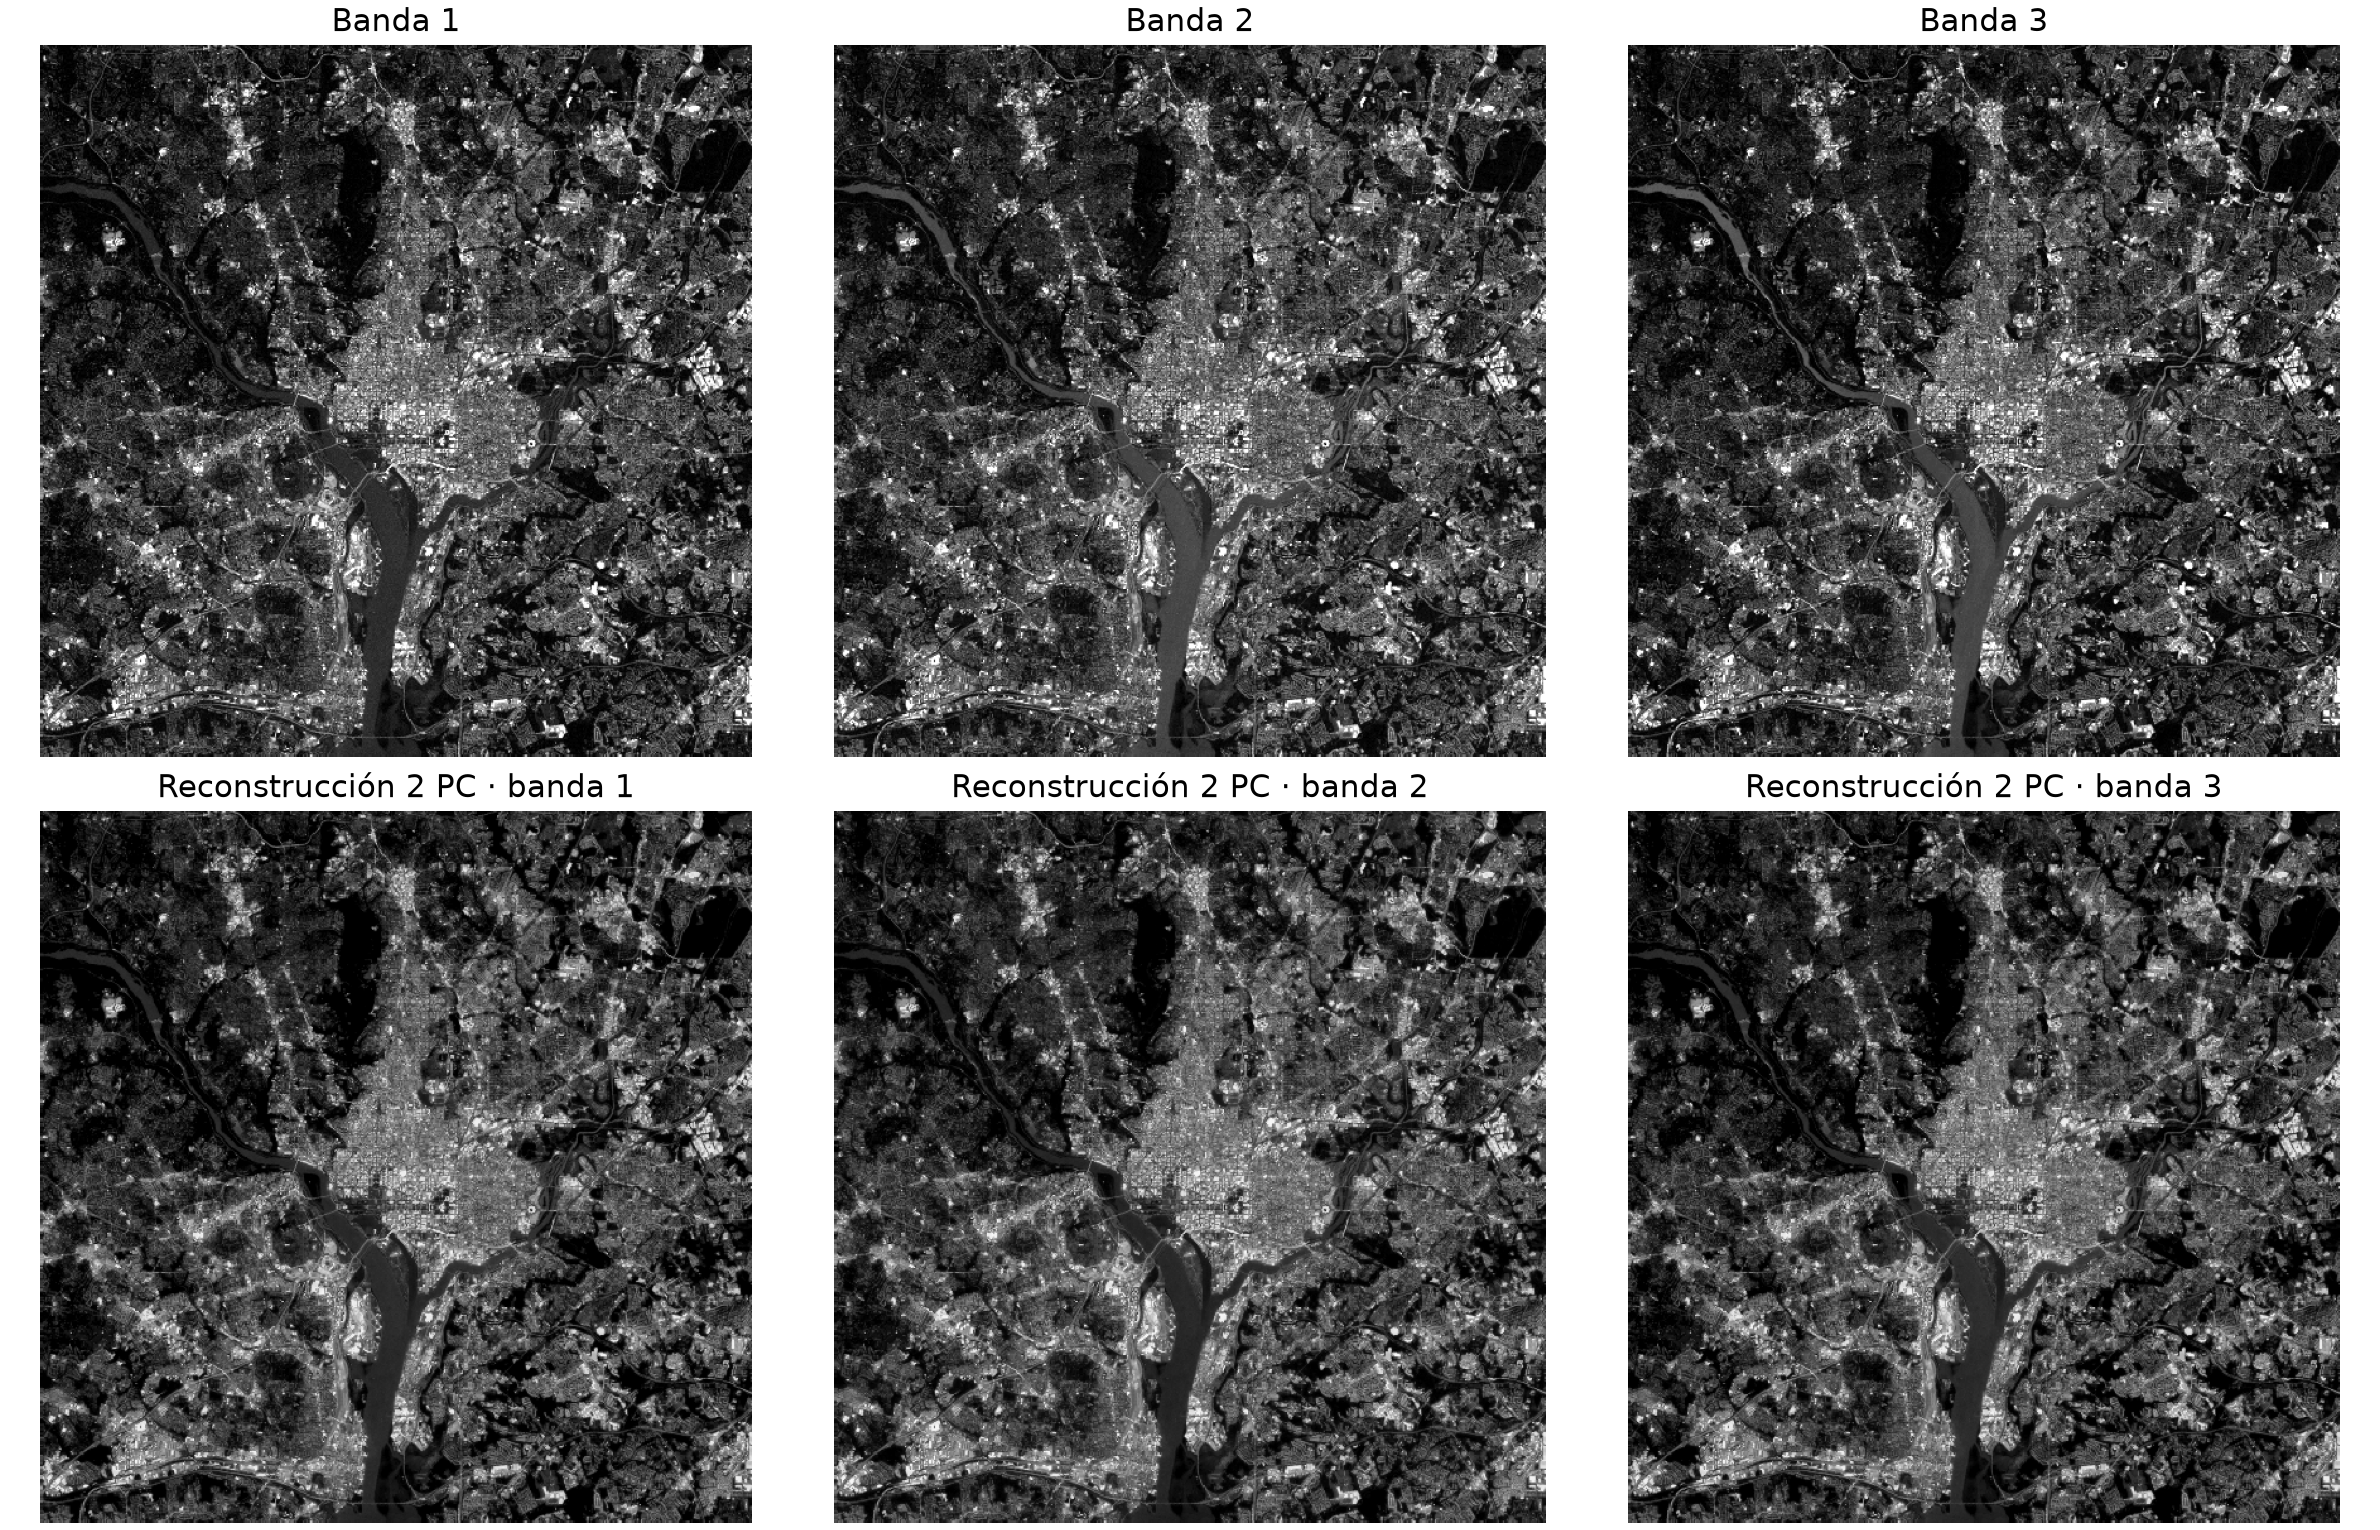
\includegraphics[width=0.9\linewidth]{washington_bandas_pca2.png}
\caption{Primeras tres bandas originales y sus reconstrucciones usando las dos primeras componentes del cubo completo.}\label{fig:bandas}\end{figure}
\begin{figure}[H]\centering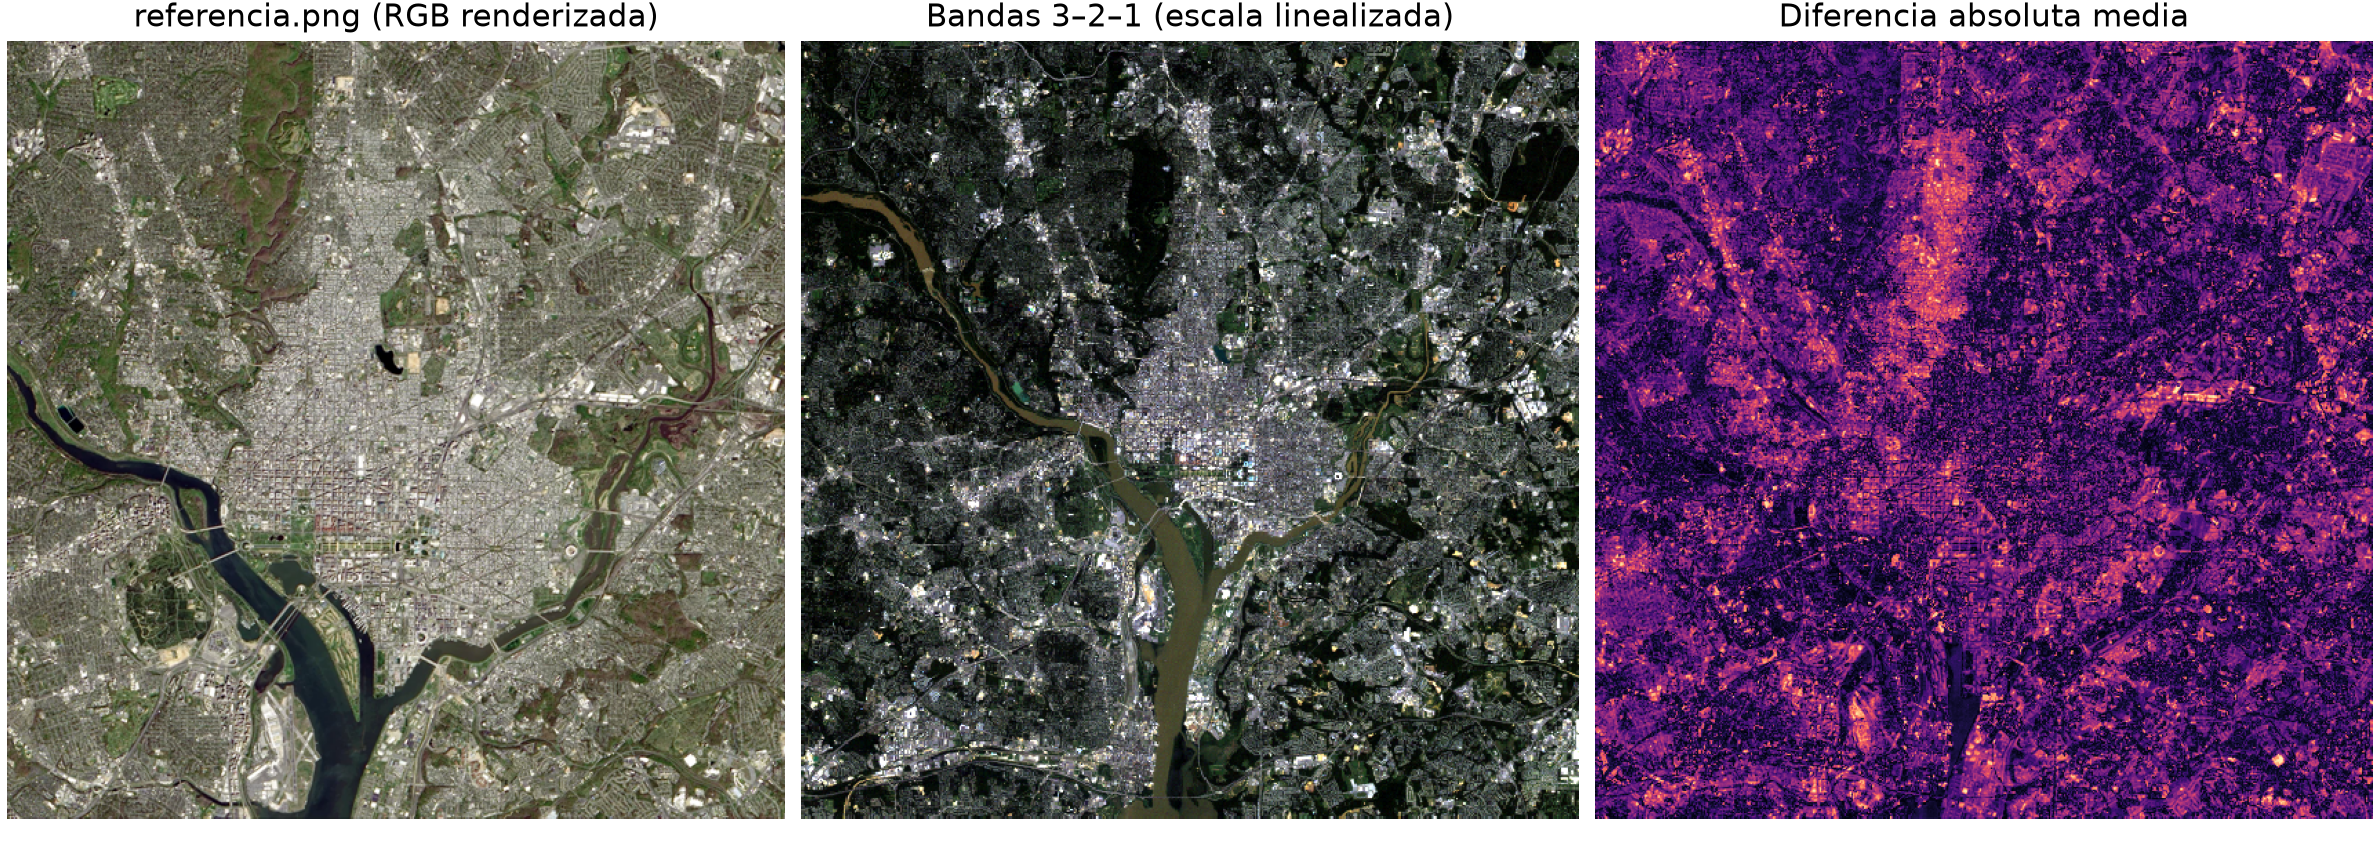
\includegraphics[width=0.92\linewidth]{referencia_vs_bandas.png}
\caption{Referencia RGB, composición 3--2--1 de las bandas y diferencia visual. La referencia es una imagen renderizada con procesamiento desconocido; no se usa como verdad de terreno radiométrica.}\label{fig:referencia}\end{figure}
`referencia.png` permite reconocer visualmente la escena. No se calcula una métrica contra la composición 3--2--1: se desconoce el procesamiento de color y contraste de referencia, así que esa diferencia no mediría la reconstrucción PCA.

\subsection{Compresión de imágenes Tokio}
La Tabla~\ref{tab:tokio} promedia por imagen las métricas de las diez escenas. Con $k=2$ se reduce a dos tercios el número de puntajes por píxel frente a RGB (factor ideal 1.5:1, más media/base).
\begin{table}[H]\centering\small
\caption{Promedio de métricas para las diez imágenes Tokio.}\label{tab:tokio}
\begin{tabular}{r r r r r}\toprule
PC retenidas & MSE & PSNR [dB] & SSIM & SAM [grados]\\\midrule
1 & 0.0087345 & 22.519 & 0.89442 & 8.8708\\
2 & 0.0021868 & 29.309 & 0.96328 & 3.8853\\
3 & $3.31\times10^{-15}$ & 146.359 & 1.00000 & 0.000004\\\bottomrule
\end{tabular}\end{table}

\begin{table}[H]\centering\small
\caption{Recuperación media de la mejora respecto al rango completo. Se requiere 90\% en cada columna.}\label{tab:recovery}
\begin{tabular}{r r r r}\toprule
PC & Reducción MSE [\%] & Ganancia SSIM [\%] & Reducción SAM [\%]\\\midrule
1 & 0.00 & 0.00 & 0.00\\
2 & 76.45 & 66.93 & 57.64\\
3 & 100.00 & 100.00 & 100.00\\\bottomrule
\end{tabular}\end{table}

Con dos componentes la recuperación no alcanza el umbral conjunto. Tres componentes sí llegan al 100\% por definición de rango completo; este es el mínimo que cumple el criterio, pero en RGB no reduce la dimensión. El resultado muestra que el umbral definido es más estricto que la impresión sugerida por las métricas brutas de la reconstrucción de dos componentes.

\begin{figure}[H]\centering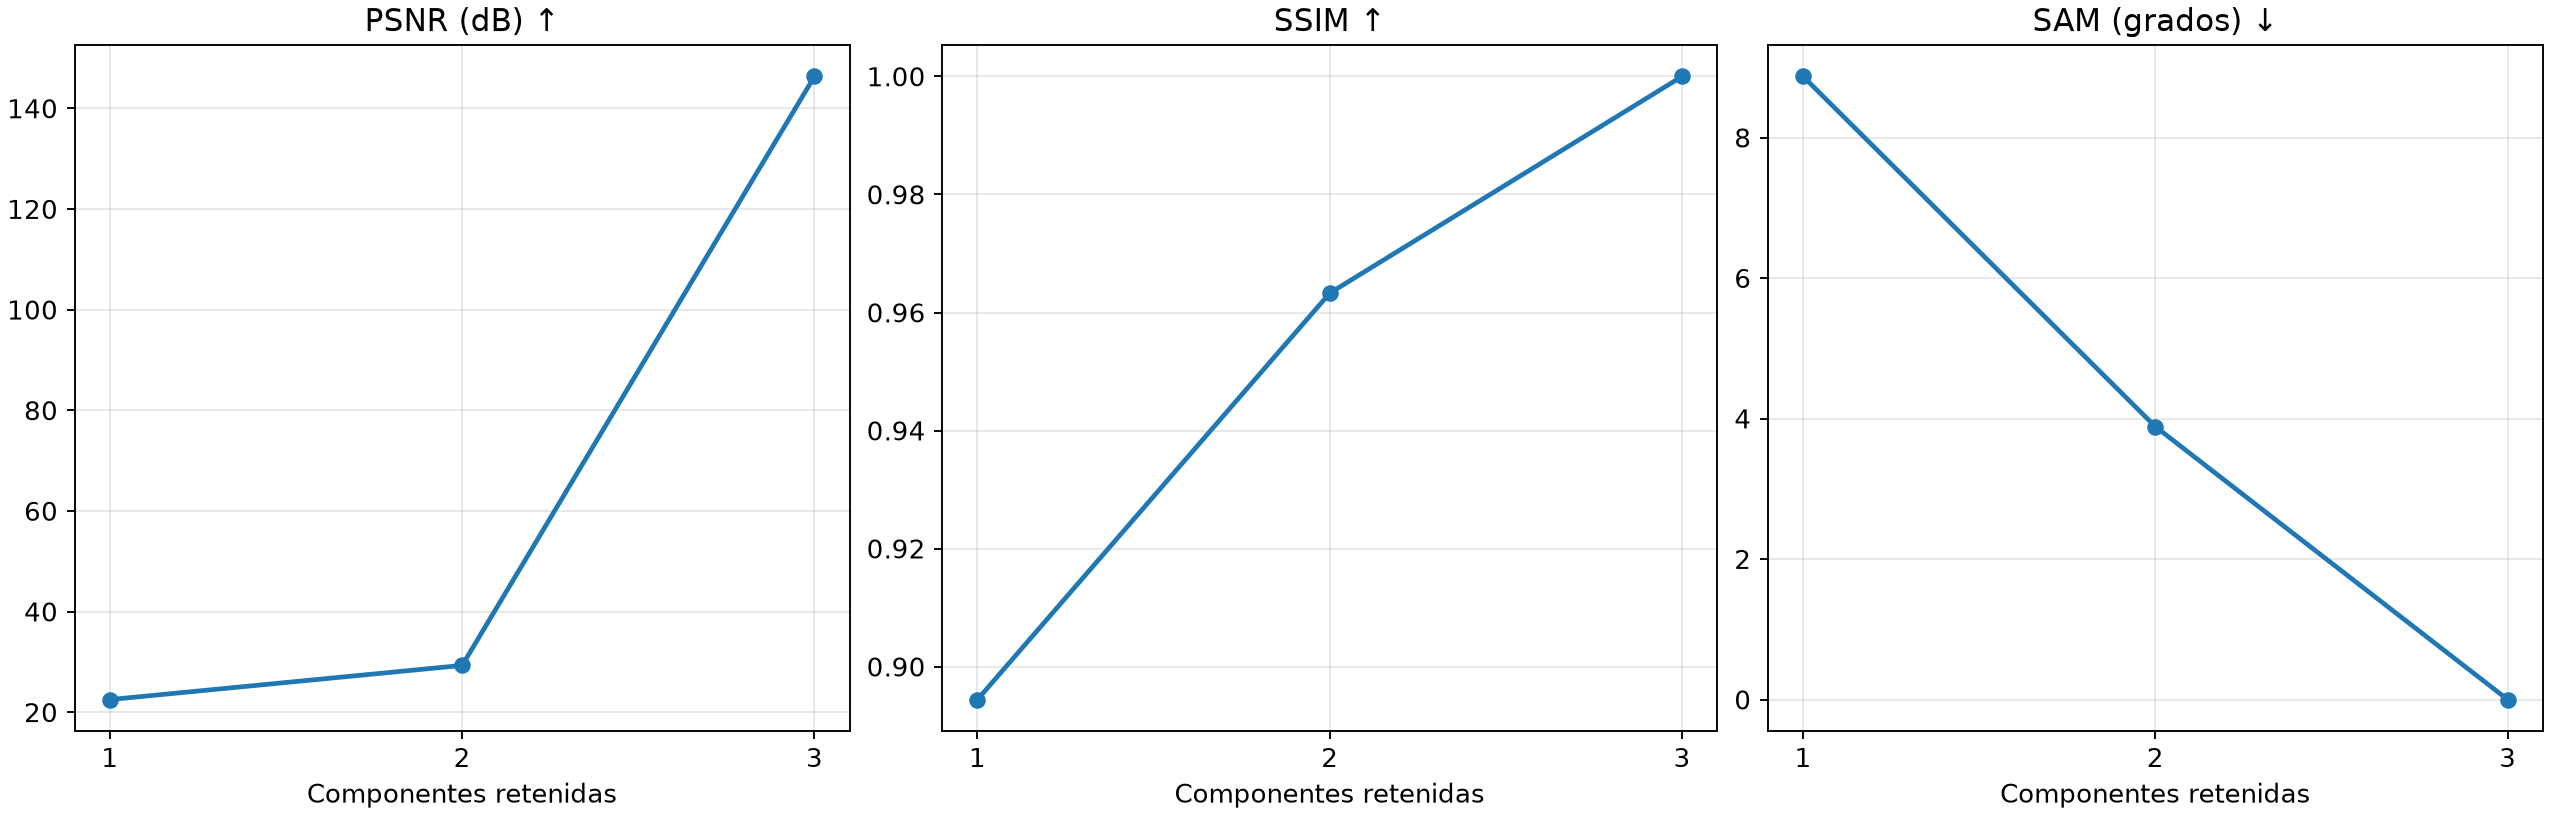
\includegraphics[width=0.9\linewidth]{metricas_tokio_pca.png}
\caption{PSNR, SSIM y SAM promedio frente al número de componentes.}\label{fig:metricas}\end{figure}
\begin{figure}[H]\centering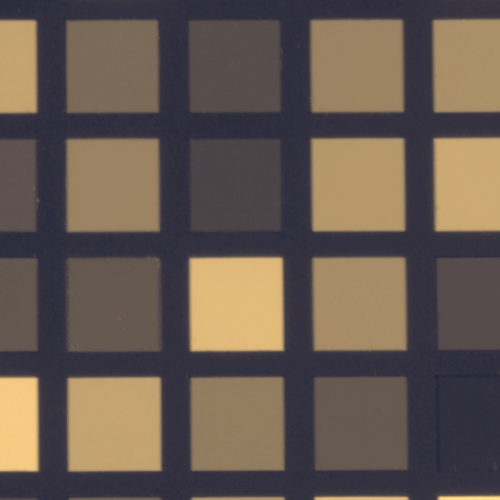
\includegraphics[width=0.68\linewidth]{colorchart_pca1.png}\hfill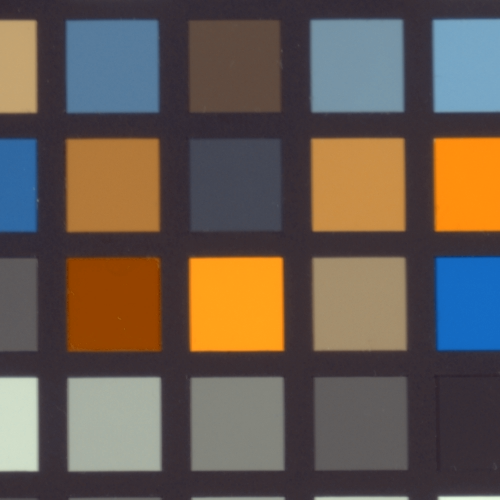
\includegraphics[width=0.29\linewidth]{colorchart_pca2.png}
\caption{Carta de color original y reconstrucción con dos componentes. La reconstrucción de una componente está disponible en el notebook.}\label{fig:colorchart}\end{figure}

\section{Discusión y conclusiones}
PCA prioriza la variación cuadrática total; no garantiza minimizar simultáneamente una métrica perceptual o espectral. En Tokio, dos componentes conservan buena similitud estructural promedio (SSIM 0.963) y PSNR 29.31 dB, con SAM 3.89°. Sin embargo, bajo la definición explícita de recuperación de mejora, se requieren tres componentes para superar 90\% en las tres métricas. JPEG ya aplica compresión y sRGB es no lineal, así que el factor informado es una reducción dimensional teórica respecto al RGB decodificado, no una tasa de bits comparada con el tamaño JPEG. El promedio de diez imágenes seleccionadas no representa las quince imágenes del directorio.

Se implementaron las ecuaciones del enunciado con covarianza poblacional, autovalores descendentes y reconstrucción centrada. En Washington D. C., dos componentes explican 88.50\% de varianza y reducen idealmente 3:1 los puntajes, con SAM de 7.55°. Debe aclararse si el curso esperaba otra definición de “90\% de exactitud”, pues la guía no especifica su denominador. El notebook oficial respalda PCA por bloques y firmas multiespectrales; Brady aporta contexto espectral. La referencia DIP que exige el enunciado aún no está disponible en el repositorio.

\section{Reproducibilidad y mejoras sugeridas}
El notebook `homework5.ipynb` se ejecutó de principio a fin. `homework5.py` genera resultados y figuras; `resultados/resultados\_pca.json` conserva los valores completos. `torch.linalg.eigh` y los productos matriciales usaron CUDA en la NVIDIA RTX 4060 Laptop GPU. El cálculo principal del script tomó 6.01 s; las métricas y figuras se calcularon en CPU. No se midió aceleración frente a CPU, por lo que se informa el backend utilizado, sin afirmar un speedup.

\begin{enumerate}[leftmargin=*]
\item \textbf{Importante:} consultar el libro DIP indicado por el enunciado (pp. 861--867) y contrastar el primer análisis con esa referencia. La copia no está en `files/`; Brady es complementario, no sustituto.
\item \textbf{Importante:} confirmar la definición de “90\% de exactitud” esperada por el profesor. El notebook deja trazable la regla adoptada y reporta las métricas brutas para recalcular si se especifica otro criterio.
\item \textbf{Opcional:} repetir el análisis Tokio con las quince imágenes o una selección aleatoria estratificada y reportar dispersión; la selección actual evita repetir la serie Butterfly.
\end{enumerate}

\end{document}

